\section {Один корень на луче}

Расположение одного корня на луче (Вариант $V$) допускает границы четырёх типов:

\begin {enumerate} [labelindent=\parindent, leftmargin=*]
    \item {$[\alpha, +\infty)$}
    \item {$(\alpha, +\infty)$}
    \item {$(-\infty, \beta]$}
    \item {$(-\infty, \beta)$}
\end {enumerate}

Для типов границ 1 и 3 возможны два особых случая: 

\begin {itemize}
    \item {существует два корня, при этом один из них попадает на включённый конец луча, а 
           второй "--- за его пределы}
    \item {существует ровно один корень, который попадает на луч }
\end {itemize}

Для типов границ 2 и 4 возможны два особых случая: 

\begin {itemize}
    \item {существует два корня, при этом один из них попадает на выколотый конец луча, а 
           второй "--- на луч}
    \item {существует ровно один корень, который попадает на луч }
\end {itemize}

\subsection {Границы типа 2}

Например, особому случаю 2 типа границ будет соответствовать следующая ситуация:

\begin {figure}[h]
    \begin {minipage} [t] {0.5\linewidth}
        \centering
        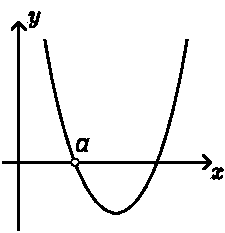
\includegraphics [width=0.6\linewidth] {image/image_12.pdf}
    \end {minipage}
    \begin {minipage} [t] {0.5\linewidth}
        \centering
        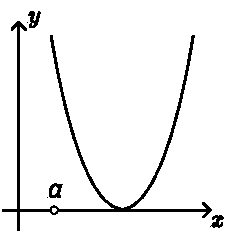
\includegraphics [width=0.6\linewidth] {image/image_14.pdf}
    \end {minipage}
\end {figure}

\subsubsection {Первый особый случай}

Первый особый случай --- существует два корня, при этом один из них попадает на выколотый конец
луча, а второй - на луч. Чтобы обработать этот случай, необходимо рассмотреть прохождение параболы
$y = f(x)$ через точку $\alpha$. То есть решить уравнение:

\begin {equation*}
    f(\alpha) = 0
\end {equation*}

Подставляем полученные параметры в трёхчлен $f(x)$ и выбираем из них те, при которых второй корень 
существует и лежит на луче $[\alpha, +\infty)$.  Это можно
сделать с помощью теоремы Виета или проверки соответствующих условий:

\begin {equation*}
    x_0 > \alpha
\end {equation*}

\subsubsection {Второй особый случай}

Второй особый случай --- существует ровно один корень, который попадает на луч. Чтобы обработать
этот особый случай, нужно рассмотреть равенство дискриминанта нулю, подставить полученные значения
параметра $p$ в трёхчлен $f(x)$ и выбрать параметры, при которых $x_0$ попадает внутрь луча
$[\alpha, +\infty)$. Это можно сделать с помощью проверки соответствующего условия:

\begin {equation*}
    x_0 > \alpha
\end {equation*}

\subsection {Границы типа 1}

\begin {figure}[h]
    \begin {minipage} [t] {\linewidth}
        \centering
        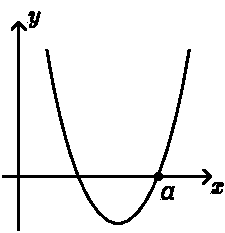
\includegraphics [width=0.3\linewidth] {image/image_19.pdf}
    \end {minipage}
\end {figure}

Разберём первый особый случай для первого типа границ (второй особый случай такой же, как и в 
предыдущем пункте).

\subsubsection {Первый особый случай}

Первый особый случай - существует два корня, при этом один из них попадает на включённый конец 
луча, а второй --- за его пределы. Чтобы обработать этот случай, необходимо рассмотреть прохождение
параболы $y = f(x)$ через точку $\alpha$. То есть решить уравнение:

\begin {equation*}
    f(\alpha) = 0
\end {equation*}

Подставляем полученные параметры в трёхчлен $f(x)$ и выбираем те, при которых второй корень 
существует и не лежит на луче $[\alpha, +\infty)$. Это можно сделать с помощью теоремы Виета или
проверки условия:

\begin {equation*}
    x_0 < \alpha
\end {equation*}

\subsection {Границы типа 1. Общий случай}

Для границ типа 1 существует два особых случая, которые описаны выше. В данном пункте на примере 
этих границ мы разберем общий случай: 

\begin {figure}[h]
    \begin {minipage} [t] {0.5\linewidth}
        \centering
        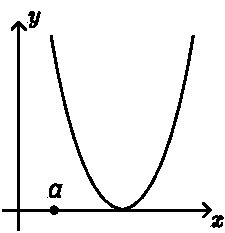
\includegraphics [width=0.6\linewidth] {image/image_20.pdf}
    \end {minipage}
    \hfill
    \begin {minipage} [t] {0.5\linewidth}
        \centering
        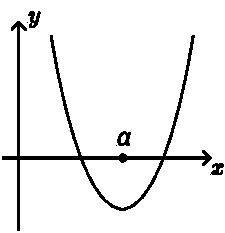
\includegraphics [width=0.6\linewidth] {image/image_21.pdf}
    \end {minipage}
\end {figure}

Чтобы ровно один корень был внутри луча $[\alpha, +\infty)$, необходимо выполнение следующих
условий:

\begin {itemize}
    \item {существует два корня}
    \item {на конце луча значение квадратного трёхчлена отрицательно (с точностью до умножения на 
           коэффициент $a$)}
\end {itemize}

Получаем следующее уравнение:

\begin {equation*}
    a \cdot f(\alpha) < 0
\end {equation*}

Как уже говорилось, чтобы получить полное решение задачи, нужно объединить особые случаи с общим 
решением.